\section{Preventing Transnational Detours}
\label{avoid_results}
In light of the results from analyzing where \textit{current} traffic is going in Section \ref{datasets}, we evaluate the effectiveness of open resolvers and relays for country avoidance.  We discuss our measurement methods, introduce an avoidance metric and algorithm, and present our findings.

\subsection{Measurement Pipelines}

{\bf Country Avoidance with Open Resolvers.} If content is replicated in different parts of the world, open DNS resolvers located around the globe can potentially help clients circumvent surveillance states.  Our measurement pipeline is shown in Figure \ref{avoidance_resolvers}.  This measurement differs slightly from that described in Section \ref{pipeline}; instead of using RIPE Atlas probes to query local DNS resolvers, we query open DNS resolvers located around the world~\cite{open_resolver_list}.  These open DNS resolvers may provide different IP addresses in the DNS responses, which represent different locations of content replicas. The measurement study in Section \ref{pipeline} used RIPE Atlas probes to traceroute to the IP addresses in DNS response, but our measurement method here uses a VPN connection to the client's country, and then traceroutes (through the VPN connection) to the IP addresses in the DNS responses given by the open resolvers.  We use a VPN connection instead of RIPE Atlas probes because of the resource limitations discussed in Section \ref{resource_limits}; because this measurement would have cost more credits than we had, we used an alternative method that still represents an Internet user in each of the five countries studied.

\begin{figure}
\centering
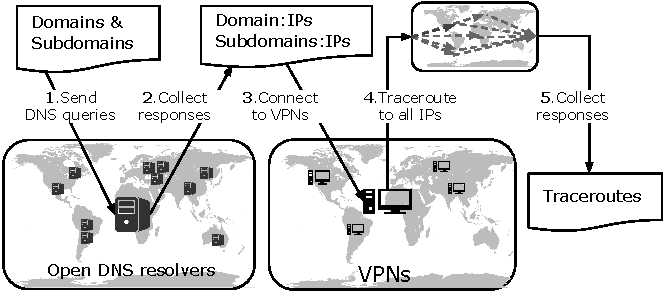
\includegraphics[width=.45\textwidth]{Country-Avoidance-Resolvers}
\caption{Measurement pipeline for country avoidance with open DNS resolvers.}
\label{fig:avoidance_resolvers}
\end{figure}

{\bf Country Avoidance with Relays.} Using an overlay network may help clients route around unfavorable countries or access content that is hosted in a more favorable country.  Figure \ref{fig:avoidance_relays} shows the steps to conduct this measurement.  After selecting relay machines, we run traceroute measurements from Country X to each relay and from each relay to the set of domains. 

\begin{figure}
\centering
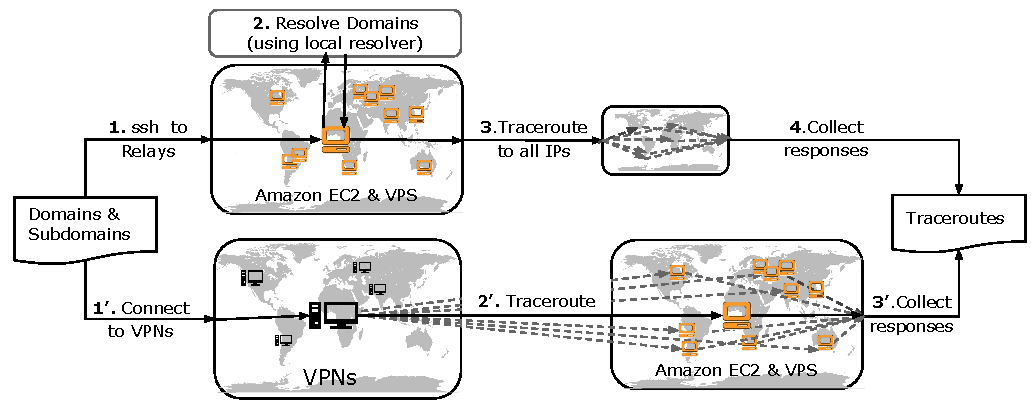
\includegraphics[width=.55\textwidth]{Country-Avoidance-Relays}
\caption{Measurement pipeline for country avoidance with overlay network relays.}
\label{fig:avoidance_relays}
\end{figure}

We use eight Amazon EC2 instances, one in each geographic region (United States, Ireland, Germany, Singapore, South Korea, Japan, Australia, Brazil), as well as 4 VPS (Virtual Private Server) machines (France, Spain, Brazil, Singapore), which are virtual machines that are functionally equivalent to dedicated physical servers.  The conjunction of these two sets of machines allow us to evaluate surveillance avoidance with a geographically diverse set of relays. By selecting an open resolver in each country that also has a relay in it we can keep the variation in measurement methods low, leading to a more accurate comparison of country avoidance methods.

\subsection{Avoidability Metrics}
\label{metrics}
We introduce a new metric and algorithm to measure how often a client in Country X can avoid a specific Country Y.  Using the proposed metric and algorithm, we can compare how well the different methods achieve country avoidance for any (Country X, Country Y) pair.

{\bf Avoidability Metric.}  This metric quantifies how often traffic can avoid Country Y when it originates in Country X.  Avoidability is explained as the fraction of paths that start in Country X and do not transit Country Y; more formally:

\[Avoidability(X,Y) = \frac{paths_{X,\bcancel{Y}}}{paths_{X}}\]

\noindent where $paths_{X,\bcancel{Y}}$ represent the paths from Country X that do not pass through Country Y, and $paths_{X}$ represent all paths that originate from Country X. The resulting value will be in the range [0,1], where 0 means the country is unavoidable for all of the domains in our study, and 1 means the client can avoid Country Y for all domains in our study.  We use this metric on country-level paths, as described in Section~\ref{pipeline}.

{\bf Avoidability Algorithm with Relays.}  Measuring the avoidability of a country Y from a client in Country X using relays has two components: 1) is Country Y on the path from the client in Country X to the relay?  2) is Country Y on the path from the relay to the domain?  For every domain, our algorithm checks if there exists at least one path from the client Country X through any relay and on to the domain, and does not transit Country Y.  The psuedo-code for the algorithm is shown in Algorithm~\ref{avoid_algo}.

\begin{algorithm}[t]
\caption{Avoidability Algorithm}
\label{avoid_algo}
\begin{algorithmic}[1]
\Function{CalcAvoidance}{set $paths1$, set $paths2$, string c}
    \State set $usableRelays$
    \For{each $(relay,path)$ in $paths1$} 
    	\If{$c$ not in $path$}
		\State $usableRelays \gets path$
	\EndIf
    \EndFor
    \State set $accessibleDomains$
    \For{each $(relay,domain,path$ in $paths2$}
    \If{$relay$ in $usableRelays$}
        \If{$c$ not in $path$}
        \State $accessibleDomains \gets domain$
        \EndIf
    \EndIf
    \EndFor
    \State $D \gets$ number of all unique domains in $paths2$
    \State $A \gets$ length of $accessibleDomains$
    \State \Return $A / D$
\EndFunction
\end{algorithmic}
\end{algorithm}

The output of the algorithm is a value in the range [0,1] that can be compared to the output of the Avoidability Metric described above.  

{\bf Upper bound on Avoidability.}  While the Avoidability metric and algorithm provide a method to quantify how avoidable Country Y is from a client in Country X, it may be the case that a number of domains are hosted in Country Y, so the Avoidance value for these countries would never reach 1.0.  For this reason, we measured the upper bound on avoidance for given pair of (Country X, Country Y) that represents the best case value for avoidance.  The pseudocode for the algorithm is shown in Algorithm \ref{upperbound_algo}.

\begin{algorithm}[t]
\caption{Avoidance Upper bound Algorithm}
\label{upperbound_algo}
\begin{algorithmic}[1]
\Function{CalcUpperbound}{set $relayDomainPaths$, string $c$}
    \State $zeros(domainLocations)$
    \For{each $(r,d,p)$ in $relayDomainPaths$} 
		\State $dest \gets $ last item in $p$
		\State $domainLocations[d] \gets dest$
    \EndFor
    \State set $accessibleDomains$
    \For{each $domain$ in $domainLocations$}
    \If{$domainLocations[domain] \neq $ set[$c$]}
    \State $accessibleDomains \gets domain$
    \EndIf
    \EndFor
    \State $D \gets$ all unique domains in  $relayDomainPaths$
    \State $A \gets$ length of $accessibleDomains$
    \State \Return $A / D$
\EndFunction
\end{algorithmic}
\end{algorithm}

The algorithm analyzes the destinations of all domains from all relays and if there exists at least one destination for a domain that is not in Country Y, then this increases the upper bound value.  An upper bound value of 1.0 means that every domain studied is hosted (or has a replica) outside of Country Y.  This value puts the Avoidance values in perspective for each (Country X, Country Y) pair. 

\subsection{Results}
After applying the metrics described in Section \ref{metrics} to country-level paths, we compared avoidance values when using open resolvers, when using relays, and when using no country avoidance tool.  First, we discuss how effective open resolvers are at country avoidance.  Then we show how effective relays are at country avoidance as well as at keeping local traffic local.  Avoidance values are shown in Table \ref{tab:avoid}, where the countries we studied are shown in the top row, and the country to avoid is in the left-most column.  

\newcolumntype{d}[1]{D{.}{.}{#1}}
\begin{table*}[t]
\centering
\begin{tabular}{|P{25mm}|d{3.2}d{3.2}|d{3.2}d{3.2}|d{3.2}d{3.2}|d{3.2}d{3.2}|d{3.2}d{3.2}|}
\multicolumn{1}{l}{}    & \headrow{No Relay} & \headrow{Relays} & \headrow{No Relay} & \headrow{Relays} & \headrow{No Relay} & \headrow{Relays}   & \headrow{No Relay} & \headrow{Relays}  & \headrow{No Relay} & \headrow{Relays} \\\hline
\textit{Country}    &\multicolumn{2}{c|}{\textit{Brazil}}   &\multicolumn{2}{c|}{\textit{Netherlands}}   &\multicolumn{2}{c|}{\textit{India}} &\multicolumn{2}{c|}{\textit{Kenya}} &\multicolumn{2}{c|}{\textit{United States}}\\
\hline\hline
Brazil               &0.00     &0.00     &1.00  &1.00   &1.00    &1.00  &1.00   &1.00  &1.00  &1.00  \\\hline\hline
Canada               &.98     &1.00     &.99  &1.00   &.98    &.98  &.99   &.99  &.92  &1.00  \\\hline
United States        &\cellcolor{blue!25}.15     &\cellcolor{blue!25}.62     &\cellcolor{blue!25}.41  &\cellcolor{blue!25}.63   &\cellcolor{blue!25}.28    &\cellcolor{blue!25}.65  &\cellcolor{blue!25}.38   &\cellcolor{blue!25}.40  &\cellcolor{blue!25}0.00  &\cellcolor{blue!25}0.00  \\\hline\hline
France               &.94     &1.00     &.89  &.99   &.89    &1.00  &.77   &.98  &.89  &.99  \\\hline
Germany              &.99     &1.00     &.95  &.99   &.96    &.99  &.95   &1.00  &.99  &1.00  \\\hline
Great Britain        &.97     &1.00     &.86  &.99   &\cellcolor{blue!25}.79    &\cellcolor{blue!25}1.00  &\cellcolor{blue!25}.50   &\cellcolor{blue!25}.97  &.99  &1.00  \\\hline
Ireland              &.97     &.99     &.89  &.99   &.96    &.99  &.86   &.99  &.99  &.99  \\\hline
Netherlands          &.98     &.99     &0.00  &0.00   &.87    &.99  &\cellcolor{blue!25}.74   &\cellcolor{blue!25}.99  &.97  &.99  \\\hline
Spain                &.82     &1.00     &.99  &.99   &1.00    &1.00  &1.00   &1.00  &1.00  &1.00  \\\hline\hline
Kenya                &1.00     &1.00     &1.00  &1.00   &1.00    &1.00  &0.00   &0.00  &1.00  &1.00  \\\hline
Mauritius            &1.00     &1.00     &1.00  &1.00   &1.00    &1.00  &\cellcolor{blue!25}.67   &\cellcolor{blue!25}.99  &1.00  &1.00  \\\hline
South Africa         &1.00     &1.00     &1.00  &1.00   &1.00    &1.00  &\cellcolor{blue!25}.66   &\cellcolor{blue!25}.66  &1.00  &1.00  \\\hline\hline
United Arab Emirates &1.00     &1.00     &1.00  &1.00   &1.00    &1.00  &.84   &.99  &1.00  &1.00  \\\hline
India                &1.00     &1.00     &.99  &1.00   &0.00    &0.00  &.94   &1.00  &.99  &1.00  \\\hline
Singapore            &.99     &1.00     &.99  &1.00   &\cellcolor{blue!25}.73    &\cellcolor{blue!25}.94  &.96   &1.00  &.99  &1.00  \\\hline
\end{tabular}
\caption{Avoidance values for different techniques of country avoidance.  The upper bound on avoidance is 1.0 in most cases, but not all.  It is 
common for some European countries to host a domain, and therefore the upper bound is slightly lower than 1.0.  The upper bound on avoidance of the 
United States is significantly lower than the upper bound on avoidance for any other country; .886, .790, .844, and .765 are the upper bounds on avoidance 
of the United States for traffic originating in Brazil, Netherlands, India, and Kenya, respectively.}
\label{tab:avoid}
\end{table*}

\subsubsection{Avoidance with Open Resolvers}
\annie{This is still being calculated, but I'll update as soon as possible.}

\subsubsection{Avoidance with Relays}
As seen in Table \ref{tab:avoid}, there are two significant trends: 1) the ability for a client to avoid a given Country Y increases with the use of relays, and 2) the least avoidable countries are surveillance states.

{\bf Avoidance Increases with Relays.}
In almost every (Country X, Country Y) pair, where Country X is the client's country (Brazil, Netherlands, India, Kenya, or the United States) and Country Y is the country to avoid, the use of an overlay network makes Country Y more avoidable than the current default routes.  The one exception we encountered is when a client is located in Kenya and wants to avoid South Africa; South Africa is on the path between the client and every relay, and therefore the client should not use the relays.  

%\begin{figure}
%\centering
%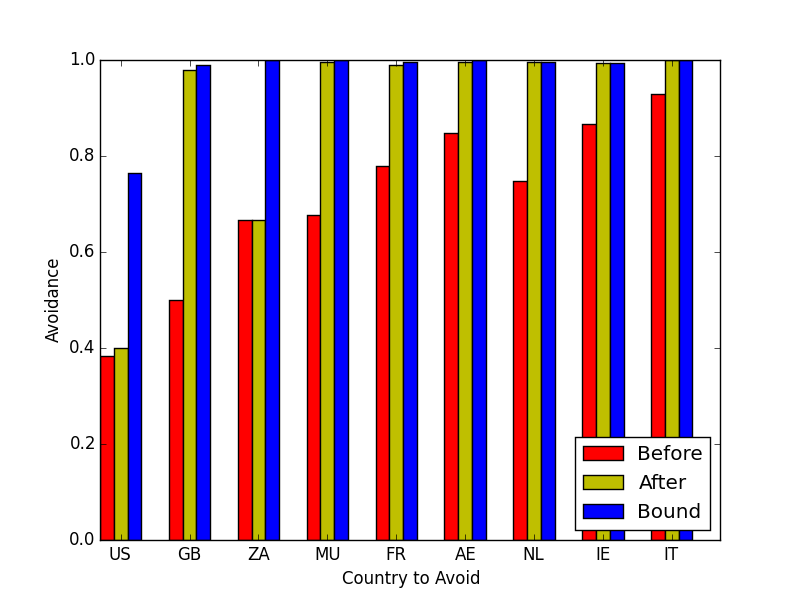
\includegraphics[width=.5\textwidth]{ke_compound_new}
%\caption{Avoidance values for Kenyan clients without relays, with relays, and the upperbound.}
%\label{fig:ke_avoidance}
%\end{figure}

For 84\% of the (Country X, Country Y) pairs shown in Table \ref{tab:avoid} the avoidance with relays reaches the upper bound on avoidance.  (Kenya, Country Y) pairs have the lowest percentage of avoidance values that reach the upper bound, showing that it is more difficult for Kenyan clients to avoid a given country.  This is not to say that relays are not effective for clients in Kenya; for example, the default routes to the top 100 domains for Kenyans avoid Great Britain 50\% of the time, but with relays this percentage increases to about 98\% of the time, and the upper bound is about 98\%. Figure \ref{fig:ke_avoidance} shows default avoidance, avoidance with relays, and the upper bound for Kenya; it's clear that despite having the worst position for avoidance out of the studied countries, in most cases the avoidance with relays either reaches or because extremely close to the upper bound.  The highest percentage (100\%) of avoidance values that reach the upper bound are for clients in the United States -- relays help clients in this country avoid all other Country Y in all cases that the domain is not hosted in Country Y.  

{\bf Surveillance States are Less Avoidable.}
Certain surveillance states discussed in Section \ref{surv} are completely unavoidable a small fraction of time from certain client locations.  France is unavoidable for a small percentage of domains for clients located in the Netherlands, Kenya, and the United States.  Similarly, clients in the Netherlands and Kenya cannot avoid Great Britain for a small fraction of domains.  

Avoidance values for (Country X, United States) pairs are significantly lower than any other Country Y for all three situations: without relays, with relays, and the upper bound.   Despite increasing clients' ability to avoid the United States, relays are not as effective at helping clients avoid this country as compared to the effectiveness of the relays at avoiding all other Country Y.  Clients in India can avoid the United States more often than clients in Brazil, Netherlands, and Kenya, with an avoidance value of .656 when using relays.  Kenyan clients can only avoid the United States 40\% of the time even while using relays.  Additionally, the upper bound for avoiding the United States is significantly lower in comparison to any other country.  

\subsubsection{Keeping Local Traffic Local}
For the cases where there were relays located in one of the five studied countries, we evaluated how effectively the use of relays kept local traffic local.  This evaluation was possible for Brazil and the United States.  In both cases, we found the percentage of tromboning traffic decreased, and the number of countries that traffic tromboned to decreased.  Tromboning Brazilian traffic decreased from 13.2\% without relays to 9.7\% with relays; when relays are used, all tromboning traffic goes only to the United States.  With the use of relays, there was only 1.3\% tromboning traffic for a United States client, whereas without relays there was 11.2\% tromboning traffic.  For the 1.2\% of traffic that trombones from the United States, it all goes only to Ireland.
